\documentclass[a4paper,11pt]{article}

%% PREAMBLE %%

% Packages
\usepackage[utf8]{inputenc} % UTF-8 is a good thing I guess
\setcounter{secnumdepth}{0}
\usepackage[a4paper, total={150mm, 225mm}]{geometry} % use reasonable amount of the page
\usepackage{amsmath}  % allows unnumbered equations
\usepackage{textcomp} % explicitly imported to calm gensymb
\usepackage{gensymb}  % gives degree sign
\usepackage{tikz}     % allows drawing pretty diagrams
\usepackage{pgfplots} % allows graphs and plots
\usepackage{graphicx} % allows images
\usepackage{pdfpages} % allows to import other PDF pages
\usepackage{float}

%Prettifying packages
\usepackage[document]{ragged2e}
\usepackage[margin=1cm]{caption} % spacing for captions, 1cm in from border
\usepackage{subcaption} 
\usepackage{fancyhdr}
\pagestyle{fancy}
\usepackage[normalem]{ulem}
\usepackage{colortbl}
\usepackage{xcolor}
\usepackage{listings}
\usepackage{tabu}

%make numbers not selectable
\usepackage{accsupp}
\renewcommand{\thelstnumber}{% Line number printing mechanism
  \protect\BeginAccSupp{ActualText={}}\arabic{lstnumber}\protect\EndAccSupp{}
}
\usepackage[T1]{fontenc}
\usepackage[framed,numbered]{matlab-prettifier} %print pretty code
\usepackage{epstopdf}

% Titlepage variables
%\title{SA1: Interim Report 1}
%\author{Paul Wernicke (pw444)\\Jonathan Collins (jc2071)}
%\date{May 2020}

\lhead{Week 2 Report}
\rhead{Jonathan Collins \& Paul Wernicke}
\lfoot{jc2071 \& pw444}

%% DOCUMENT %%
\pagenumbering{gobble}
\begin{document}
%\maketitle
\begin{titlepage}
    \begin{center}
 
        \LARGE
        SA1: Aircraft Wing Analysis
        
        \vspace{0.1cm}
        
        \LARGE
        
        Interim Report 1
        
        \vspace{0.4cm}
        
        \large
        
        Jonathan Collins \& Paul Wernicke
        
        \vspace{0cm}
        
        Homerton College
        
        \vspace{0.3cm}
        
        Easter Term 2020
        
        \vspace{0.5cm}
        
        %\large
        
        %\textbf{Abstract}
        
        %\justify
        
        %\normalsize
        %I don't think we really need an abstract.
        %\tableofcontents
        \lstlistoflistings
    \end{center}
\end{titlepage}
\pagenumbering{arabic}

\section{Exercise 1}
% Lising of ueintbit.m
\lstinputlisting[style= Matlab-editor,basicstyle = \mlttfamily,label=ueintbit,
  caption=ueintbit.m]{ueintbit.m}

%listing of script
\lstinputlisting[style= Matlab-editor,basicstyle = \mlttfamily, caption=Exercise 1 script]{Week_2_master/exercise1.m}

% momentum thickness plot

\section{Exercise 2}
% listing of refpaninf.m
\lstinputlisting[style= Matlab-editor,basicstyle = \mlttfamily,label=refpaninf,
  caption=refpaninf.m]{refpaninf.m}

% listing of script
\lstinputlisting[style= Matlab-editor,basicstyle = \mlttfamily,label=script2,
  caption=Exercise 2 script]{Week_1_pw444/exercise2.m}
  
%four contour plots, showing exact and approximate values of fa,fb

\begin{figure}[htbp]
\centering
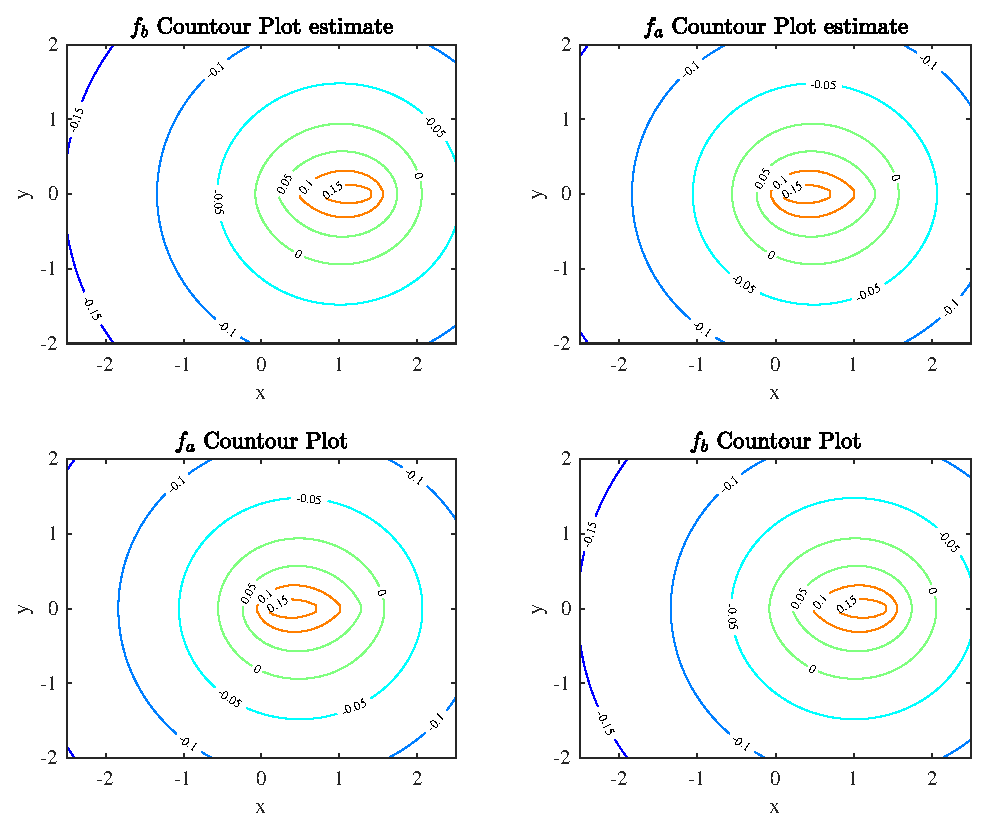
\includegraphics[scale=0.90]{Exercise_2_Contourplots.eps}
\caption{Exercise 1.}
\label{Exercise 2}
\end{figure}

\section{Exercise 3}
% listing of refpaninf.m
\lstinputlisting[style= Matlab-editor,basicstyle = \mlttfamily,label=panelinf,
  caption=panelinf.m]{panelinf.m}
  
\pagebreak

% listing of script
\lstinputlisting[style= Matlab-editor,basicstyle = \mlttfamily,label=script3,
  caption=Exercise 3 script]{Week_1_master/exercise3.m}

% four contour plots, showing exact and approximate values of fa,fb
% contour plot of fa
\begin{figure}[H]
\centering
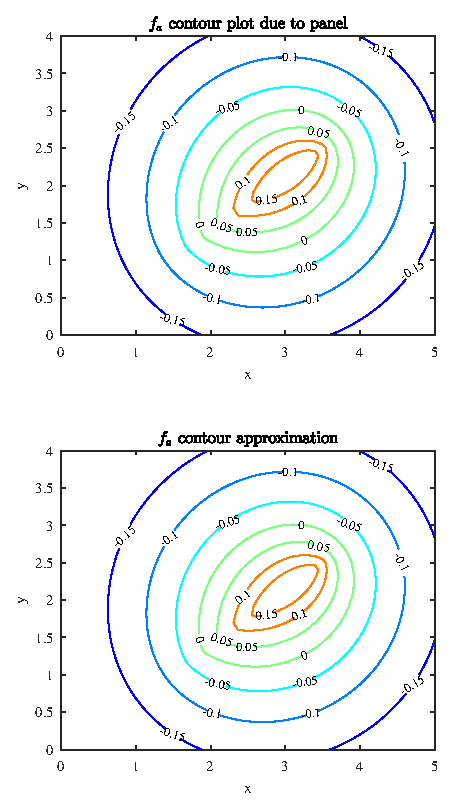
\includegraphics[scale=1.55]{graphs/e3g1.eps}
\caption{Contour plots of $f_a$ for a general vortex-sheet-panel, showing both exact and approximate values}
\label{e3g1}
\end{figure}
% contour plot of fb
\begin{figure}[H]
\centering
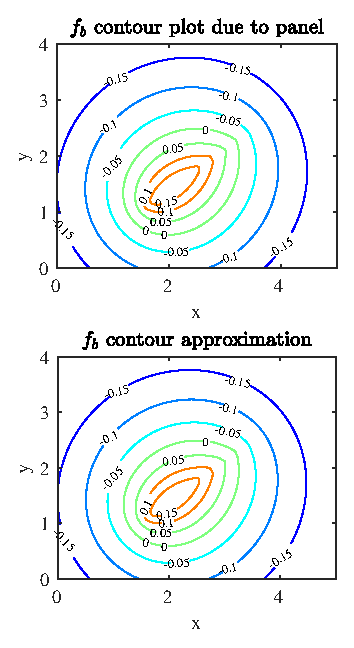
\includegraphics[scale=1.55]{graphs/e3g2.eps}
\caption{Contour plots of $f_b$ for a general vortex-sheet-panel, showing both exact and approximate values}
\label{e3g2}
\end{figure}


\section{Exercise 4}
% Listing of thickdash.m
\lstinputlisting[style= Matlab-editor,basicstyle = \mlttfamily, caption=thickdash.m]{thickdash.m}

% listing of script
\lstinputlisting[style= Matlab-editor,basicstyle = \mlttfamily, caption=Exercise 4 script]{Week_2_master/exercise4.m}

% results graph
\begin{figure}[H]
\centering
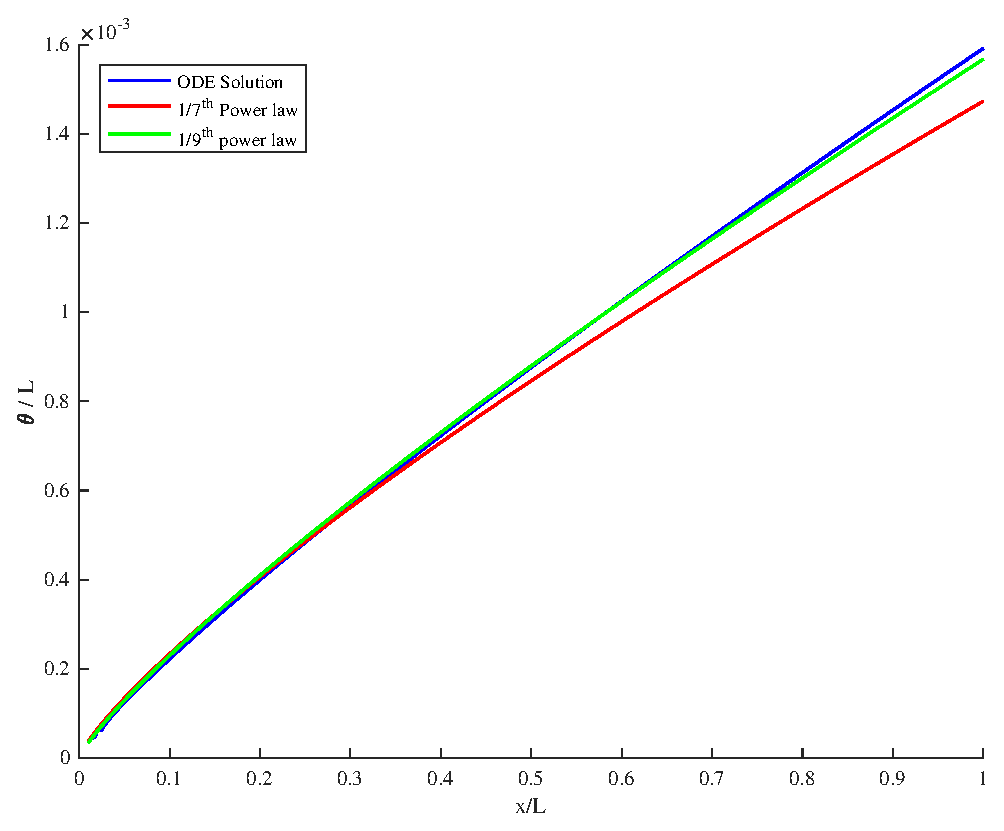
\includegraphics[scale=0.70]{graphs/e4g1.eps}
\caption{}
\label{e4g1}
\end{figure}

\section{Exercise 5}
% listing of build_lhs.m
\lstinputlisting[style= Matlab-editor,basicstyle = \mlttfamily,label=buildlhs,
  caption=build\_lhs.m]{build_lhs.m}

% listing of build_rhs.m
\lstinputlisting[style= Matlab-editor,basicstyle = \mlttfamily,label=buildrhs,
  caption=build\_rhs.m]{build_rhs.m}
  
% listing of script
\lstinputlisting[style= Matlab-editor,basicstyle = \mlttfamily,label=script5,
  caption=Exercise 5 script]{Week_1_master/exercise5.m}

%plot of surface velocity α = 0
\begin{figure}[htbp]
\centering
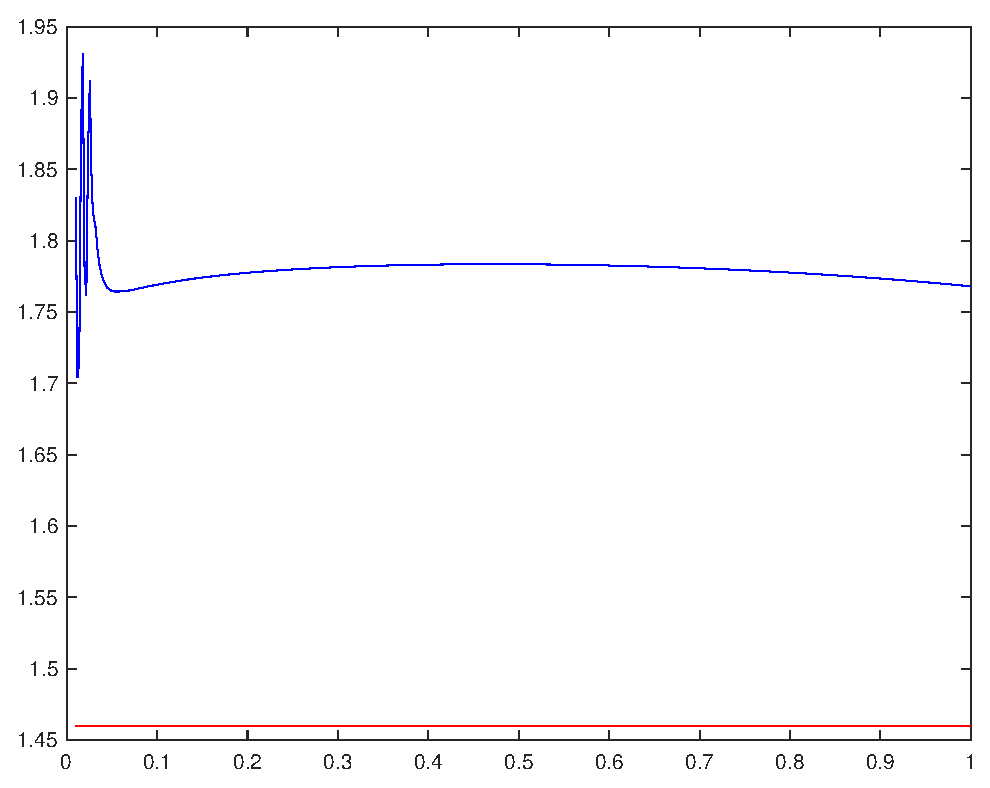
\includegraphics[scale=0.65]{graphs/e5g1.eps}
\caption{Circulation over cylinder surface at $\alpha = 0$}
\label{e5g1}
\end{figure}

%plot of surface velocity α = π/18
\begin{figure}[htbp]
\centering
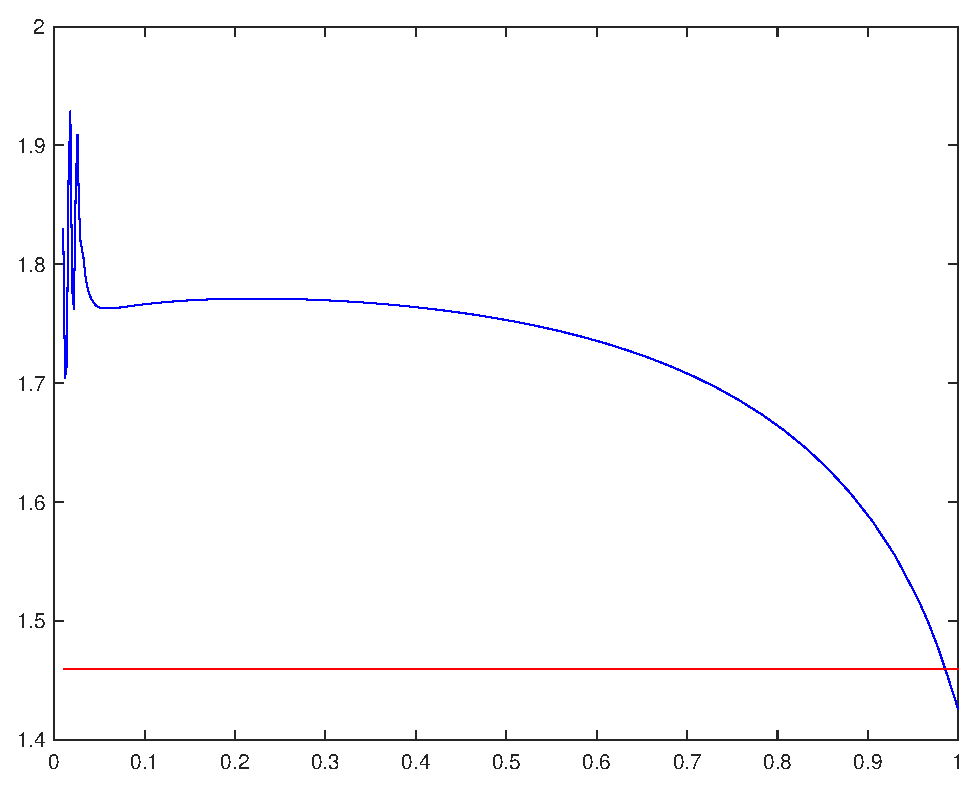
\includegraphics[scale=0.65]{graphs/e5g2.eps}
\caption{Circulation over cylinder surface at $\alpha = \pi/18$}
\label{e5g1}
\end{figure}

\justify
\vspace{1cm}
For the case when $\alpha = \pi/18$:
\[
\Gamma = -2.1828
\]



\section{Exercise 6}
% tikz flowchart

% listing of script
\lstinputlisting[style= Matlab-editor,basicstyle = \mlttfamily,
  caption=Exercise 6 script]{Week_2_master/exercise6.m}

% four plots as specified
\begin{figure}[H]
\centering
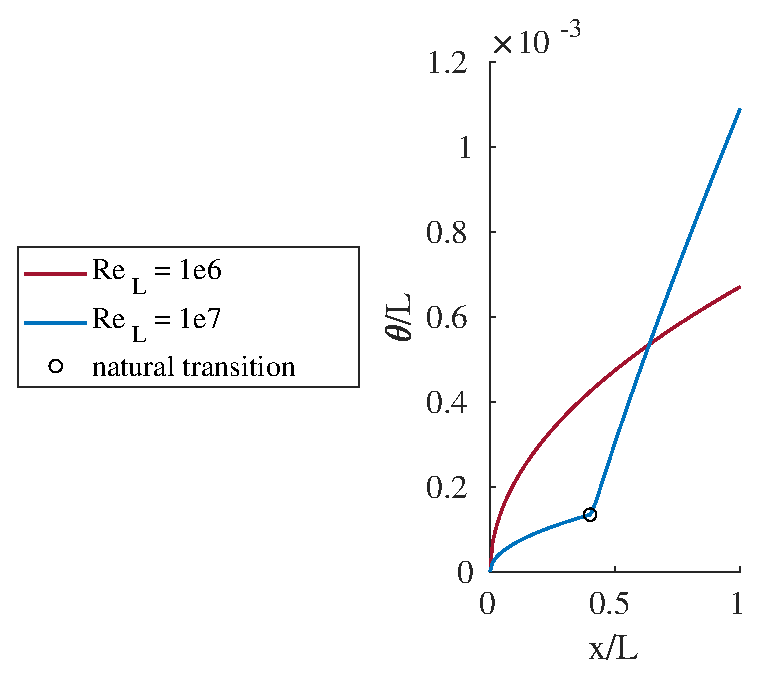
\includegraphics[scale=0.8]{graphs/e6g1.eps}
\caption{}
\label{e6g1}
\end{figure}

\begin{figure}[H]
\centering
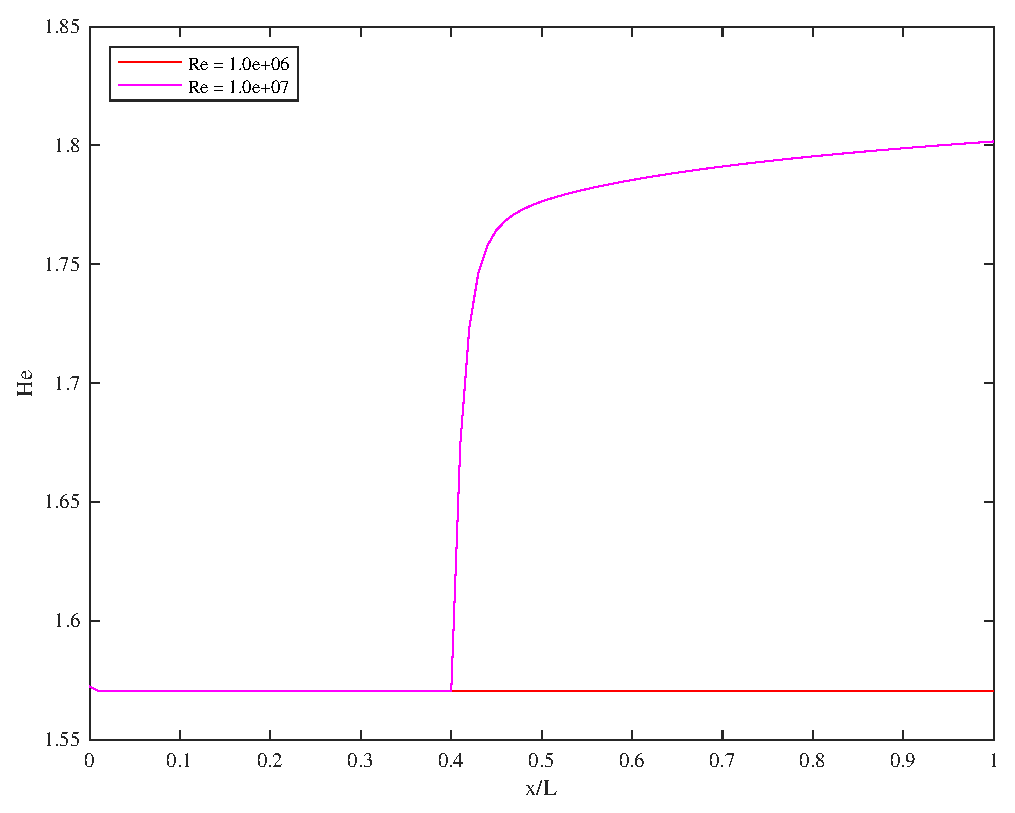
\includegraphics[scale=0.8]{graphs/e6g2.eps}
\caption{}
\label{e6g2}
\end{figure}

\begin{figure}[H]
\centering
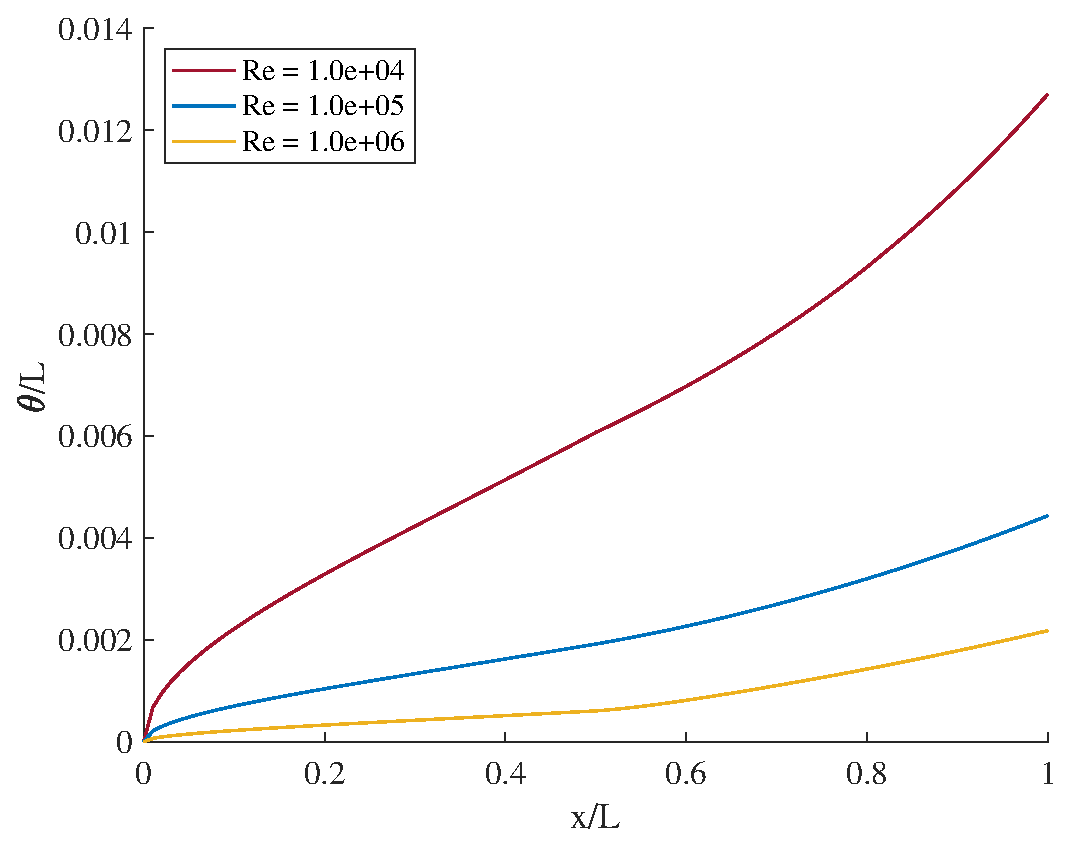
\includegraphics[scale=0.8]{graphs/e6g3.eps}
\caption{}
\label{e6g3}
\end{figure}

\begin{figure}[H]
\centering
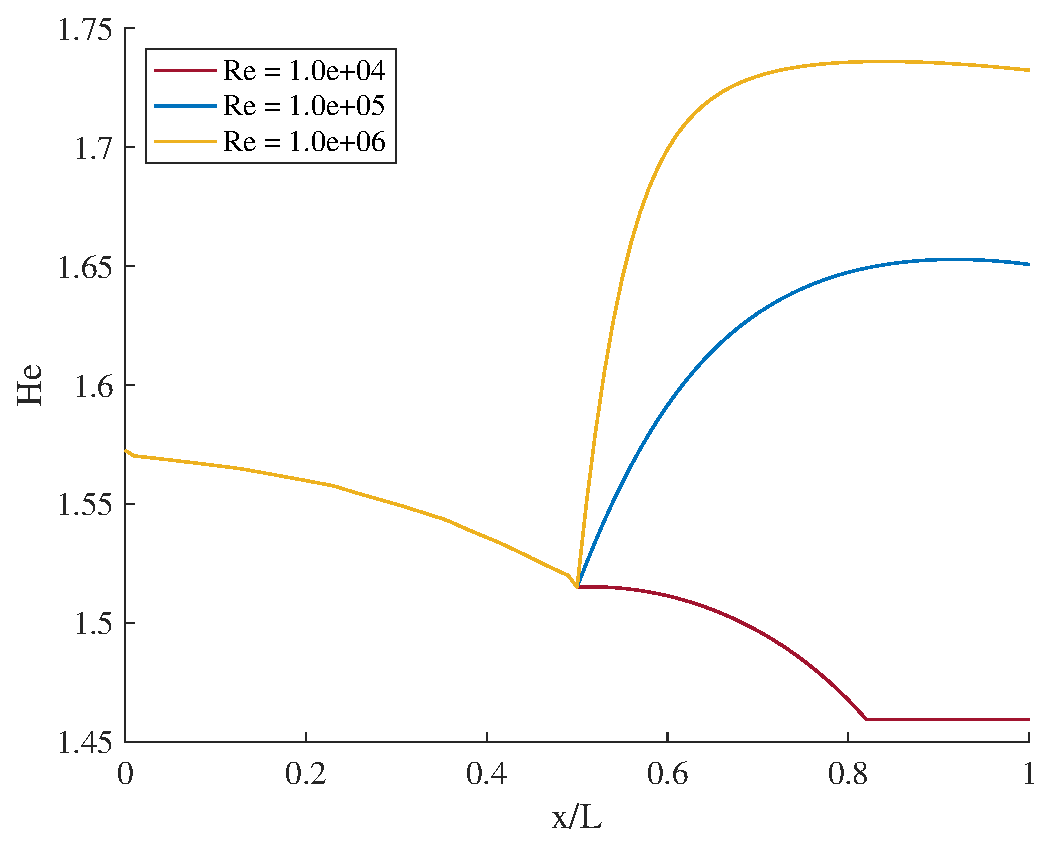
\includegraphics[scale=0.8]{graphs/e6g4.eps}
\caption{}
\label{e6g4}
\end{figure}

% critical velocity gradient as specified




\tikzset{every picture/.style={line width=0.75pt}} %set default line width to 0.75pt        

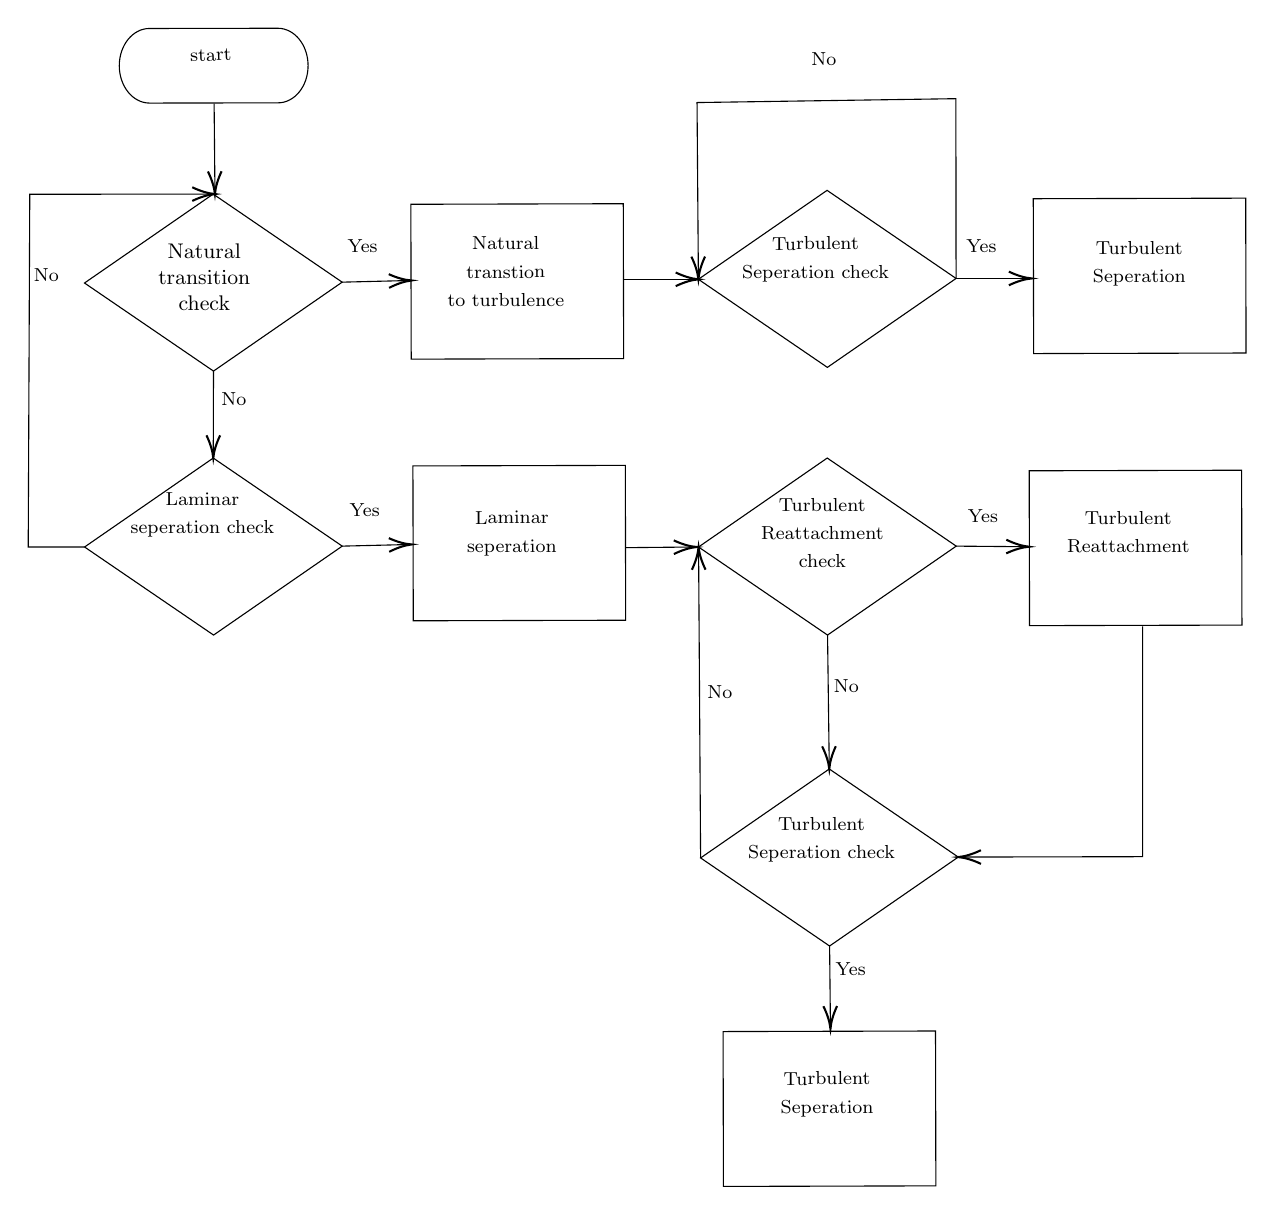
\begin{tikzpicture}[x=0.75pt,y=0.75pt,yscale=-1,xscale=1]
%uncomment if require: \path (0,734); %set diagram left start at 0, and has height of 734

%Flowchart: Terminator [id:dp7207071910268746] 
\draw   (67.63,154.62) -- (129.49,154.51) .. controls (137.52,154.5) and (144.06,162.53) .. (144.09,172.46) .. controls (144.12,182.38) and (137.62,190.44) .. (129.59,190.45) -- (67.73,190.56) .. controls (59.7,190.57) and (53.16,182.54) .. (53.13,172.61) .. controls (53.1,162.69) and (59.6,154.63) .. (67.63,154.62) -- cycle ;
%Straight Lines [id:da10986730772092312] 
\draw    (98.82,190.8) -- (99.21,232.4) ;
\draw [shift={(99.22,234.4)}, rotate = 269.47] [color={rgb, 255:red, 0; green, 0; blue, 0 }  ][line width=0.75]    (10.93,-3.29) .. controls (6.95,-1.4) and (3.31,-0.3) .. (0,0) .. controls (3.31,0.3) and (6.95,1.4) .. (10.93,3.29)   ;
%Straight Lines [id:da11218528639690684] 
\draw    (98.52,319.7) -- (98.41,359.58) ;
\draw [shift={(98.41,361.58)}, rotate = 270.15] [color={rgb, 255:red, 0; green, 0; blue, 0 }  ][line width=0.75]    (10.93,-3.29) .. controls (6.95,-1.4) and (3.31,-0.3) .. (0,0) .. controls (3.31,0.3) and (6.95,1.4) .. (10.93,3.29)   ;
%Flowchart: Decision [id:dp47636663676641755] 
\draw   (98.41,361.58) -- (160.55,404.02) -- (98.56,446.87) -- (36.41,404.44) -- cycle ;
%Flowchart: Process [id:dp0035186106511891913] 
\draw   (193.61,239.32) -- (295.96,239.05) -- (296.13,313.66) -- (193.78,313.93) -- cycle ;
%Straight Lines [id:da41405154544556755] 
\draw    (160.52,276.84) -- (191.97,276.07) ;
\draw [shift={(193.97,276.03)}, rotate = 538.61] [color={rgb, 255:red, 0; green, 0; blue, 0 }  ][line width=0.75]    (10.93,-3.29) .. controls (6.95,-1.4) and (3.31,-0.3) .. (0,0) .. controls (3.31,0.3) and (6.95,1.4) .. (10.93,3.29)   ;
%Straight Lines [id:da4839414628019604] 
\draw    (36.41,404.44) -- (9.26,404.43) -- (10,234.5) -- (97.22,234.4) ;
\draw [shift={(99.22,234.4)}, rotate = 539.94] [color={rgb, 255:red, 0; green, 0; blue, 0 }  ][line width=0.75]    (10.93,-3.29) .. controls (6.95,-1.4) and (3.31,-0.3) .. (0,0) .. controls (3.31,0.3) and (6.95,1.4) .. (10.93,3.29)   ;
%Straight Lines [id:da47695648438676885] 
\draw    (295.76,275.47) -- (330.14,275.47) ;
\draw [shift={(332.14,275.47)}, rotate = 180] [color={rgb, 255:red, 0; green, 0; blue, 0 }  ][line width=0.75]    (10.93,-3.29) .. controls (6.95,-1.4) and (3.31,-0.3) .. (0,0) .. controls (3.31,0.3) and (6.95,1.4) .. (10.93,3.29)   ;
%Flowchart: Decision [id:dp5291766920258706] 
\draw   (98.37,234.4) -- (160.52,276.84) -- (98.52,319.69) -- (36.37,277.25) -- cycle ;
%Flowchart: Process [id:dp6243738863575946] 
\draw   (194.6,365.38) -- (296.94,365.11) -- (297.11,439.72) -- (194.77,439.99) -- cycle ;

%Flowchart: Process [id:dp6109994002876044] 
\draw   (493.49,236.64) -- (595.83,236.37) -- (596,310.98) -- (493.66,311.25) -- cycle ;
%Flowchart: Decision [id:dp19310726941760736] 
\draw   (394.14,232.61) -- (456.29,275.05) -- (394.29,317.9) -- (332.14,275.46) -- cycle ;
%Flowchart: Decision [id:dp374284511592351] 
\draw   (395.21,511.39) -- (457.35,553.83) -- (395.35,596.68) -- (333.21,554.24) -- cycle ;
%Flowchart: Decision [id:dp9780902027233841] 
\draw   (394.22,361.58) -- (456.37,404.02) -- (394.37,446.87) -- (332.22,404.44) -- cycle ;
%Straight Lines [id:da6310642789542652] 
\draw    (160.55,404.02) -- (192.01,403.26) ;
\draw [shift={(194.01,403.21)}, rotate = 538.61] [color={rgb, 255:red, 0; green, 0; blue, 0 }  ][line width=0.75]    (10.93,-3.29) .. controls (6.95,-1.4) and (3.31,-0.3) .. (0,0) .. controls (3.31,0.3) and (6.95,1.4) .. (10.93,3.29)   ;
%Straight Lines [id:da12370255545736619] 
\draw    (456.29,275.05) -- (490.66,275.05) ;
\draw [shift={(492.66,275.05)}, rotate = 180] [color={rgb, 255:red, 0; green, 0; blue, 0 }  ][line width=0.75]    (10.93,-3.29) .. controls (6.95,-1.4) and (3.31,-0.3) .. (0,0) .. controls (3.31,0.3) and (6.95,1.4) .. (10.93,3.29)   ;
%Straight Lines [id:da6933448349630812] 
\draw    (297.08,404.76) -- (329.24,404.45) ;
\draw [shift={(331.24,404.44)}, rotate = 539.46] [color={rgb, 255:red, 0; green, 0; blue, 0 }  ][line width=0.75]    (10.93,-3.29) .. controls (6.95,-1.4) and (3.31,-0.3) .. (0,0) .. controls (3.31,0.3) and (6.95,1.4) .. (10.93,3.29)   ;
%Straight Lines [id:da4268759513220136] 
\draw    (456.29,275.05) -- (456.2,188.44) -- (331.49,190.31) -- (332.13,273.47) ;
\draw [shift={(332.14,275.47)}, rotate = 269.56] [color={rgb, 255:red, 0; green, 0; blue, 0 }  ][line width=0.75]    (10.93,-3.29) .. controls (6.95,-1.4) and (3.31,-0.3) .. (0,0) .. controls (3.31,0.3) and (6.95,1.4) .. (10.93,3.29)   ;
%Straight Lines [id:da994392836584868] 
\draw    (394.37,446.87) -- (395.18,509.39) ;
\draw [shift={(395.2,511.39)}, rotate = 269.26] [color={rgb, 255:red, 0; green, 0; blue, 0 }  ][line width=0.75]    (10.93,-3.29) .. controls (6.95,-1.4) and (3.31,-0.3) .. (0,0) .. controls (3.31,0.3) and (6.95,1.4) .. (10.93,3.29)   ;
%Straight Lines [id:da857618285731965] 
\draw    (456.37,404.02) -- (489.42,404.3) ;
\draw [shift={(491.42,404.31)}, rotate = 180.47] [color={rgb, 255:red, 0; green, 0; blue, 0 }  ][line width=0.75]    (10.93,-3.29) .. controls (6.95,-1.4) and (3.31,-0.3) .. (0,0) .. controls (3.31,0.3) and (6.95,1.4) .. (10.93,3.29)   ;
%Straight Lines [id:da4592324807700441] 
\draw    (395.36,596.68) -- (395.75,634.57) ;
\draw [shift={(395.77,636.57)}, rotate = 269.4] [color={rgb, 255:red, 0; green, 0; blue, 0 }  ][line width=0.75]    (10.93,-3.29) .. controls (6.95,-1.4) and (3.31,-0.3) .. (0,0) .. controls (3.31,0.3) and (6.95,1.4) .. (10.93,3.29)   ;
%Flowchart: Process [id:dp46735660020681147] 
\draw   (344.04,637.9) -- (446.39,637.63) -- (446.55,712.24) -- (344.21,712.51) -- cycle ;
%Flowchart: Process [id:dp5152442854440118] 
\draw   (491.52,367.72) -- (593.86,367.45) -- (594.03,442.06) -- (491.69,442.33) -- cycle ;
%Straight Lines [id:da7889844522327492] 
\draw    (333.21,554.24) -- (332.24,406.44) ;
\draw [shift={(332.23,404.44)}, rotate = 449.62] [color={rgb, 255:red, 0; green, 0; blue, 0 }  ][line width=0.75]    (10.93,-3.29) .. controls (6.95,-1.4) and (3.31,-0.3) .. (0,0) .. controls (3.31,0.3) and (6.95,1.4) .. (10.93,3.29)   ;
%Straight Lines [id:da7830600664422521] 
\draw    (546.2,442.63) -- (546.2,553.64) -- (459.35,553.82) ;
\draw [shift={(457.35,553.83)}, rotate = 359.88] [color={rgb, 255:red, 0; green, 0; blue, 0 }  ][line width=0.75]    (10.93,-3.29) .. controls (6.95,-1.4) and (3.31,-0.3) .. (0,0) .. controls (3.31,0.3) and (6.95,1.4) .. (10.93,3.29)   ;

% Text Node
\draw (162.01,255.44) node [anchor=north west][inner sep=0.75pt]  [rotate=-359.86,xscale=0.85,yscale=0.85] [align=left] {{\footnotesize Yes}};
% Text Node
\draw (101.21,329.24) node [anchor=north west][inner sep=0.75pt]  [rotate=-359.86,xscale=0.85,yscale=0.85] [align=left] {{\footnotesize No}};
% Text Node
\draw (460.19,255.43) node [anchor=north west][inner sep=0.75pt]  [rotate=-359.86,xscale=0.85,yscale=0.85] [align=left] {{\footnotesize Yes}};
% Text Node
\draw (10.92,269.42) node [anchor=north west][inner sep=0.75pt]  [rotate=-359.86,xscale=0.85,yscale=0.85] [align=left] {{\footnotesize No}};
% Text Node
\draw (350.18,254.04) node [anchor=north west][inner sep=0.75pt]  [rotate=-359.86,xscale=0.85,yscale=0.85] [align=left] {\begin{minipage}[lt]{65.779375pt}\setlength\topsep{0pt}
\begin{center}
{\footnotesize Turbulent \ }\\{\footnotesize Seperation check}
\end{center}

\end{minipage}};
% Text Node
\draw (86.09,164.01) node [anchor=north west][inner sep=0.75pt]  [font=\small,rotate=-358.05,xscale=0.85,yscale=0.85] [align=left] {{\footnotesize start}};
% Text Node
\draw (55.17,257.54) node [anchor=north west][inner sep=0.75pt]  [font=\small,rotate=-359.86,xscale=0.85,yscale=0.85] [align=left] {\begin{minipage}[lt]{66.671875pt}\setlength\topsep{0pt}
\begin{center}
{\small Natural transition }\\{\small check}
\end{center}

\end{minipage}};
% Text Node
\draw (55.55,377.21) node [anchor=north west][inner sep=0.75pt]  [rotate=-359.86,xscale=0.85,yscale=0.85] [align=left] {\begin{minipage}[lt]{64.419375pt}\setlength\topsep{0pt}
\begin{center}
{\footnotesize Laminar}\\{\footnotesize seperation check}
\end{center}

\end{minipage}};
% Text Node
\draw (202.74,253.99) node [anchor=north west][inner sep=0.75pt]  [rotate=-359.86,xscale=0.85,yscale=0.85] [align=left] {\begin{minipage}[lt]{62.591875pt}\setlength\topsep{0pt}
\begin{center}
{\footnotesize Natural transtion}\\{\footnotesize  to turbulence}
\end{center}

\end{minipage}};
% Text Node
\draw (218.02,386.11) node [anchor=north west][inner sep=0.75pt]  [rotate=-359.86,xscale=0.85,yscale=0.85] [align=left] {\begin{minipage}[lt]{40.831875000000004pt}\setlength\topsep{0pt}
\begin{center}
{\footnotesize Laminar }\\{\footnotesize seperation}
\end{center}

\end{minipage}};
% Text Node
\draw (162.99,382.51) node [anchor=north west][inner sep=0.75pt]  [rotate=-359.86,xscale=0.85,yscale=0.85] [align=left] {{\footnotesize Yes}};
% Text Node
\draw (519.57,256.06) node [anchor=north west][inner sep=0.75pt]  [rotate=-359.86,xscale=0.85,yscale=0.85] [align=left] {\begin{minipage}[lt]{42.191875pt}\setlength\topsep{0pt}
\begin{center}
{\footnotesize Turbulent \ }\\{\footnotesize Seperation}
\end{center}

\end{minipage}};
% Text Node
\draw (359.14,379.97) node [anchor=north west][inner sep=0.75pt]  [rotate=-359.86,xscale=0.85,yscale=0.85] [align=left] {\begin{minipage}[lt]{55.791875000000005pt}\setlength\topsep{0pt}
\begin{center}
{\footnotesize Turbulent \ }\\{\footnotesize Reattachment }\\{\footnotesize check}
\end{center}

\end{minipage}};
% Text Node
\draw (385.51,165.09) node [anchor=north west][inner sep=0.75pt]  [rotate=-359.86,xscale=0.85,yscale=0.85] [align=left] {{\footnotesize No}};
% Text Node
\draw (353.09,533.57) node [anchor=north west][inner sep=0.75pt]  [rotate=-359.86,xscale=0.85,yscale=0.85] [align=left] {\begin{minipage}[lt]{65.779375pt}\setlength\topsep{0pt}
\begin{center}
{\footnotesize Turbulent }\\{\footnotesize Seperation check}
\end{center}

\end{minipage}};
% Text Node
\draw (396.33,467.37) node [anchor=north west][inner sep=0.75pt]  [rotate=-359.86,xscale=0.85,yscale=0.85] [align=left] {{\footnotesize No}};
% Text Node
\draw (507.83,386.19) node [anchor=north west][inner sep=0.75pt]  [rotate=-359.86,xscale=0.85,yscale=0.85] [align=left] {\begin{minipage}[lt]{53.52875pt}\setlength\topsep{0pt}
\begin{center}
{\footnotesize Turbulent }\\{\footnotesize Reattachment}
\end{center}

\end{minipage}};
% Text Node
\draw (460.9,385.18) node [anchor=north west][inner sep=0.75pt]  [rotate=-359.86,xscale=0.85,yscale=0.85] [align=left] {{\footnotesize Yes}};
% Text Node
\draw (397.14,603.54) node [anchor=north west][inner sep=0.75pt]  [rotate=-359.86,xscale=0.85,yscale=0.85] [align=left] {{\footnotesize Yes}};
% Text Node
\draw (369.13,656.31) node [anchor=north west][inner sep=0.75pt]  [rotate=-359.86,xscale=0.85,yscale=0.85] [align=left] {\begin{minipage}[lt]{42.191875pt}\setlength\topsep{0pt}
\begin{center}
{\footnotesize Turbulent \ }\\{\footnotesize Seperation}
\end{center}

\end{minipage}};
% Text Node
\draw (335.37,470.05) node [anchor=north west][inner sep=0.75pt]  [rotate=-359.86,xscale=0.85,yscale=0.85] [align=left] {{\footnotesize No}};


\end{tikzpicture}


\section{Auxiliary Functions}
We have used one auxiliary function in our code from the MATLAB File Exchange. The function is called \textbf{legendUnq} and allows plot legends to show only unique entries. The function can be found online here: 


Adam Danz (2020). legendUnq (https://www.mathworks.com/matlabcentral/fileexchange/67646-legendunq), MATLAB Central File Exchange. Retrieved May 18, 2020. 


It is also listed below.
\lstinputlisting[style= Matlab-editor,basicstyle = \mlttfamily,
  caption=legendUnq.m]{legendUnq.m}

\end{document}